\begin{table}[htbp]
\centering\small
\caption{午夜保持与六小时更新的预测误差}\label{tab:q3-prediction}
\begin{tabular}{llrrrr}
\toprule
变量 & 版本 & MAE/kW & MSE/$\mathrm{kW}^2$ & RMSE/kW & $R^2$\\
\midrule
负载 & 午夜保持 & 144.77 & 37,193.15 & 192.86 & 0.9812\\
负载 & 日内更新 & 139.61 & 33,887.37 & 184.09 & 0.9829\\
光伏 & 午夜保持 & 198.89 & 143,999.34 & 379.47 & 0.9840\\
光伏 & 日内更新 & 91.24 & 29,493.09 & 171.74 & 0.9967\\
净需求 & 午夜保持 & 288.13 & 183,992.27 & 428.94 & 0.9699\\
净需求 & 日内更新 & 187.21 & 63,403.78 & 251.80 & 0.9896\\
\bottomrule
\end{tabular}
\end{table}
\begin{table}[htbp]
\centering\small
\caption{规划场景与实际执行的独立核验}\label{tab:q3-verification}
\begin{tabular}{lr}
\toprule
检查项目 & 结果\\
\midrule
最大供需残差/kWh & 1.42e-13\\
最大SOC递推残差/kWh & 9.09e-13\\
最大逐槽计费残差/元 & 9.09e-13\\
跨日SOC断点/kWh & 0.00e+00\\
实际同时充放电槽数 & 0\\
实际紧急电充电槽数 & 0\\
所有规划场景最大充放重叠/kWh & 2.58e-08\\
所有规划场景最大充电与紧急电重叠/kWh & 2.13e-07\\
求解次数（含一月） & 1460\\
平均/最大相对间隙 & 3.228\% / 565.092\%\\
限时结束次数 & 499\\
\bottomrule
\end{tabular}
\end{table}
全部实际轨迹通过物理与计费核验，但部分规划限时终止，不能据此认定经济最优。日内目标省略已付原计划常数，并包含退款和终端库存项；其相对间隙可能较大，不等同于年度真实费用的相对误差。仅午夜对照的平均与最大间隙分别为4.842\%和35.457\%；主方案与对照的完整回放用时分别为1606.60\,s和748.16\,s，均不含HGB训练。
\begin{table}[htbp]
\centering\small
\caption{误差路径尺度的四季指定日敏感性}\label{tab:q3-sensitivity}
\begin{tabular}{lrrr}
\toprule
$\kappa$ & 四日总费用/元 & 相对变化/\% & 紧急购电量/kWh\\
\midrule
0.9 & 165,836.03 & -0.061 & 667.43\\
1.0 & 165,936.77 & +0.000 & 669.69\\
1.1 & 166,992.37 & +0.636 & 487.84\\
\bottomrule
\end{tabular}
\end{table}
在上述四个指定日及同日初状态条件下，误差尺度上下浮动10\%时，费用最大偏移为0.636\%。这一结果衡量局部风险参数敏感性；固定秒数预算下可行解也可能变化，不将有限日期的结果推广为任意天气或跨年度的稳定性保证。
\begin{table}[htbp]
\centering\small
\caption{相同预测输入层下的信息更新策略对照}\label{tab:q3-comparison}
\begin{tabular}{lrrr}
\toprule
方案 & 实际总费用/元 & 紧急购电/kWh & 非空换向/次\\
\midrule
仅午夜计划 & 13,773,732.21 & 97,553.83 & 6057\\
六小时滚动更新 & 12,972,155.14 & 38,802.76 & 6029\\
\bottomrule
\end{tabular}
\end{table}
完整策略对照中，日内更新相对仅午夜计划减少费用801,577.08元，变化比例为5.820\%。两组均从1月1日6000\,kWh开始独立预热，2月1日初始库存分别为1779.833与1903.010\,kWh，因此该比较反映包括预热和后续重规划在内的完整策略差异，不是固定二月初态的单因素因果估计。是否保留每一次发布，还需在相同起点下逐次删除更新机会；本实验不据总体比较断言每个更新时间都必要。
\begin{figure}[htbp]
\centering
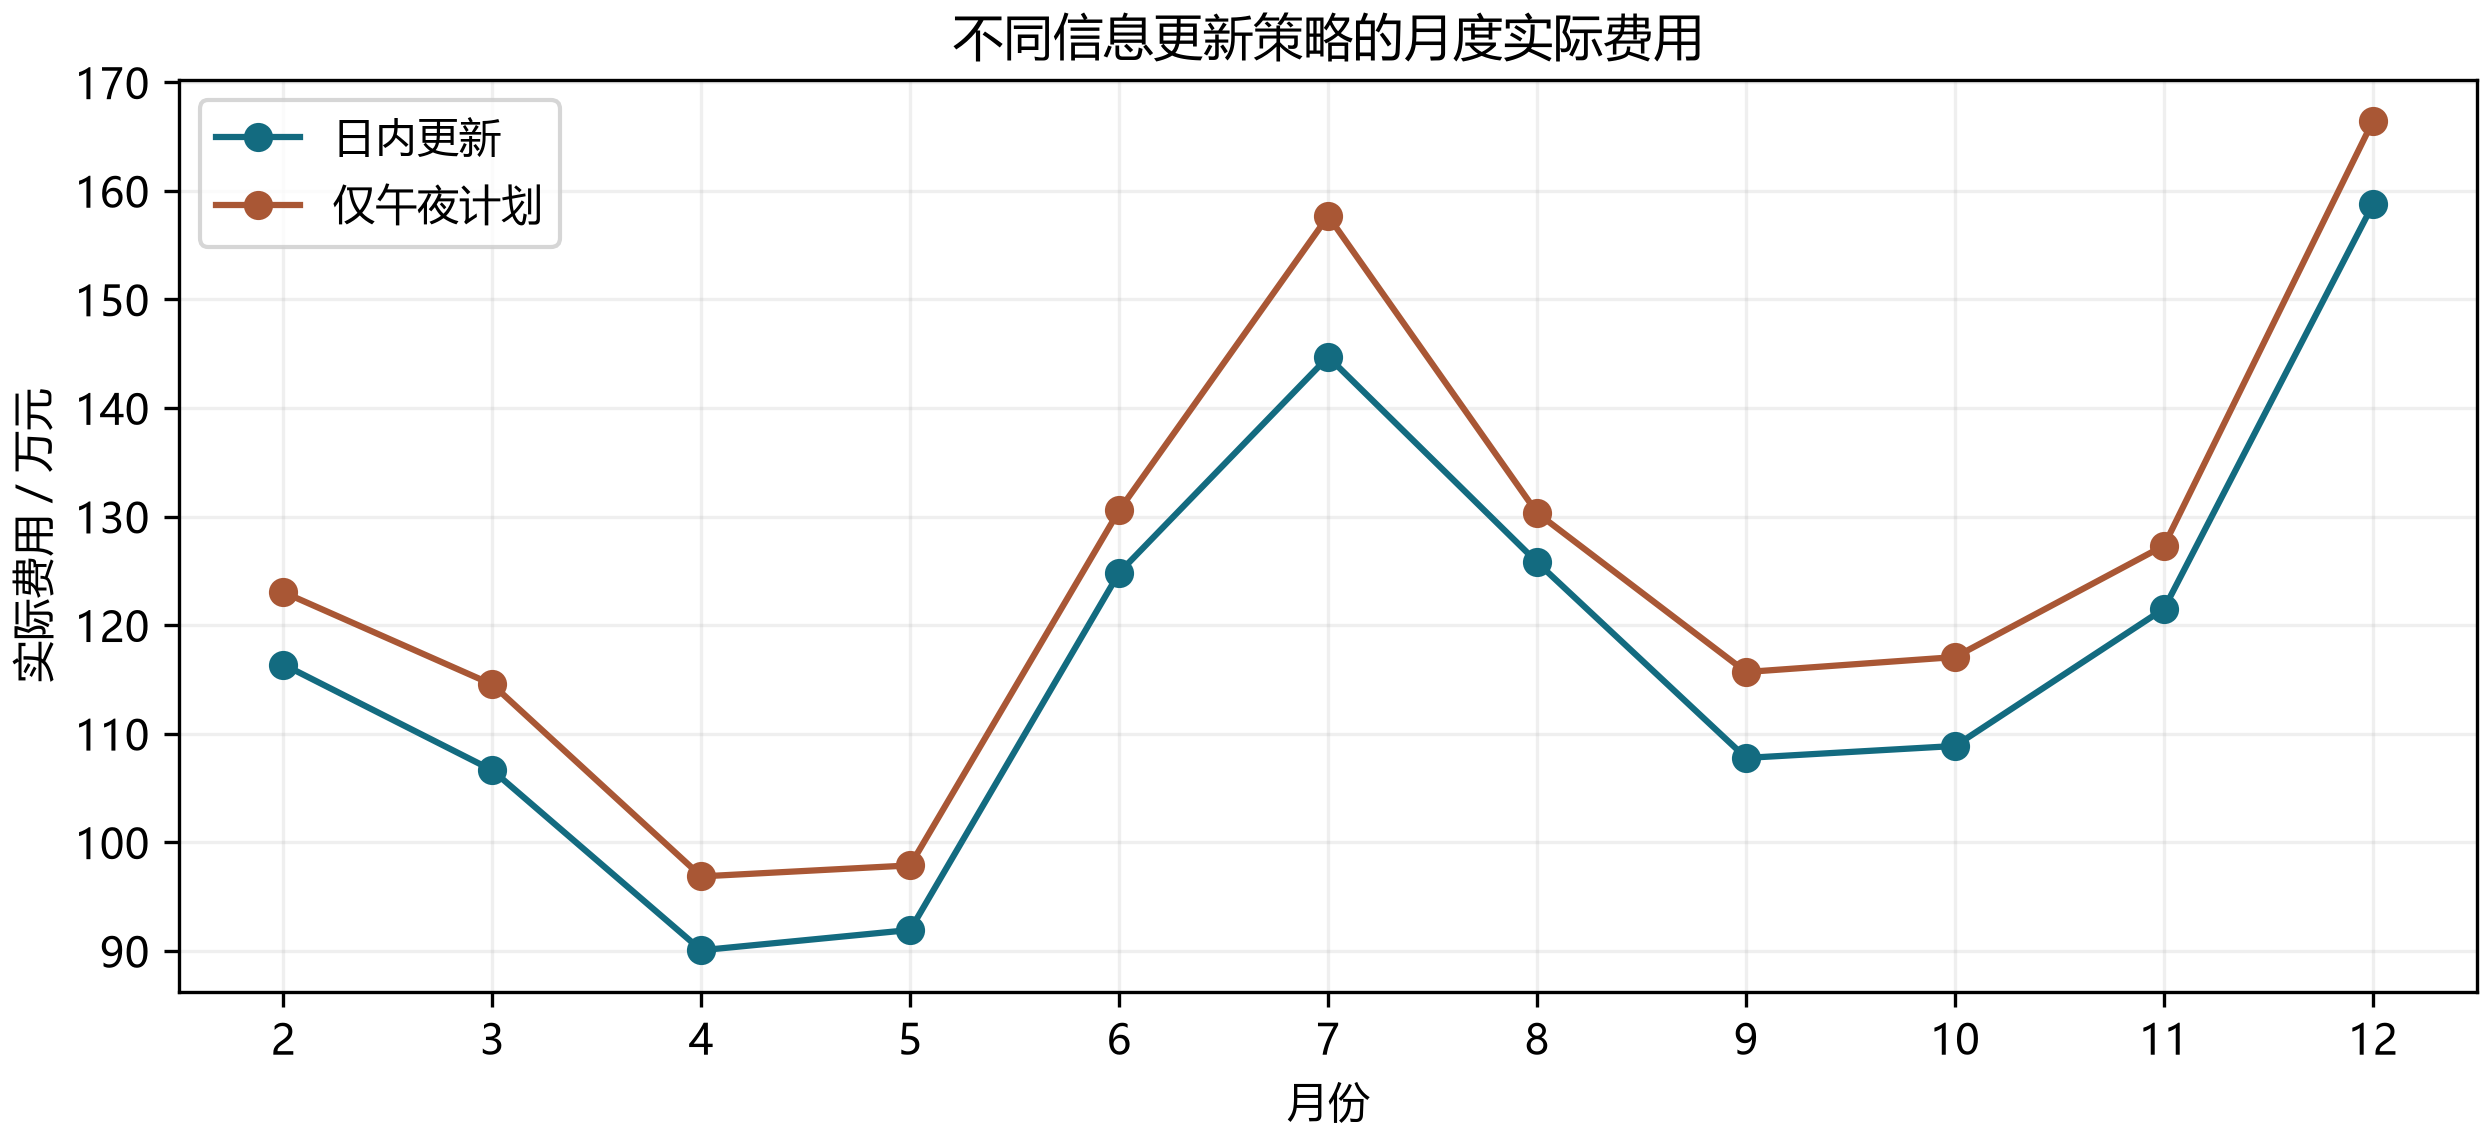
\includegraphics[width=.86\textwidth]{q3_run/paper/q3_monthly.png}
\caption{日内更新与仅午夜计划的月度实际费用}\label{fig:q3-monthly}
\parbox{.94\textwidth}{\footnotesize 图注：按相同结算公式逐槽累加月度费用，两组独立传递实际库存，展示更新策略的季节性费用差异。}
\end{figure}
两组单次规划均限时2秒，但更新方案每天求解4次，午夜对照仅求解1次；且限时MILP的最优间隙针对各自代理目标，不能作为年度实际费用的最优性保证。因此上述差额是给定求解预算下的策略实测差异，并不把信息、计算投入和解质量的影响完全分离。2025年数据已用于此前模型开发，故本次属于按时间推进的开发年度评价。物理核验和未来扰动检查支持实现的一致性与信息边界，但不构成未触碰测试集、全局最优或电池延寿证明。
